% autore: Andrea Ciprietti

\createsection{\Soluzione}{{\small{$\blacksquare$}} \normalsize Soluzione del problema}
\createsection{\Codice}{{\small{$\blacksquare$}} \normalsize Codice della soluzione (\texttt{C++})}

    Questo semplice problema può essere risolto con complessità e consumo di memoria costanti.
    
    \Soluzione

    L'idea di base consiste nel distinguere alcuni casi da risolvere separatamente.
    
    Ad esempio, è possibile che che il costo di $M$ biglietti singoli non superi quello del carnet: in questo caso, acquistare un carnet da $M$ biglietti di costo $B$ risulterebbe sconveniente rispetto a comperare $M$ biglietti al prezzo di $A$ centesimi ciascuno (o, nel migliore dei casi, le due scelte sarebbero equivalenti). È chiaro, dunque, che in questo caso la scelta migliore consiste nell'acquistare $N$ biglietti singoli.
    
    Supponiamo ora che un carnet sia più conveniente di $M$ biglietti (e cioè, che valga la disuguaglianza $B < M \cdot A$). Siano $q$ ed $r$ il quoziente e il resto della divisione euclidea tra $N$ ed $M$ ($q,r \in \mathbb{N} \: : \: N = q \cdot M + r, \; 0 \le r < M$). Allora, la spesa ottimale si ha acquistando $q$ carnet, più la scelta di costo minore tra $r$ biglietti singoli o un ulteriore carnet. Moralmente, infatti, non stiamo facendo altro che raggruppare i biglietti a $M$ a $M$, in modo da procurarci i biglietti di ciascun gruppo con un singolo carnet, e infine acquistare nel modo migliore i biglietti restanti.
    
    \Codice
    
    \colorbox{white}{\makebox[.99\textwidth][l]{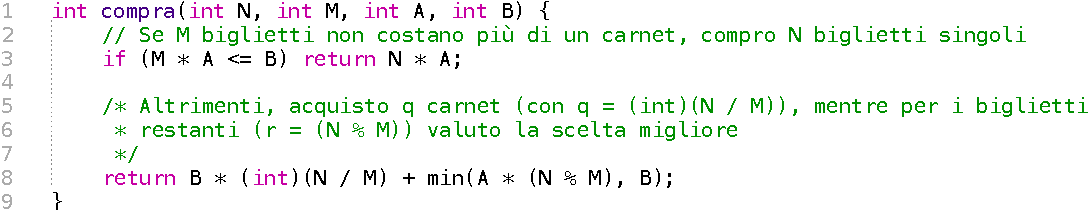
\includegraphics[scale=.8]{biglietti_sol.pdf}}}